\makeatletter
\makeatother
\documentclass[10pt,english]{article}\usepackage{graphicx, color}
%% maxwidth is the original width if it is less than linewidth
%% otherwise use linewidth (to make sure the graphics do not exceed the margin)
\usepackage{alltt}
\usepackage[T1]{fontenc}
\usepackage[latin9]{inputenc}
\usepackage{geometry}
\geometry{left=1.5cm,right=1.5cm,top=2cm,bottom=2cm}
\usepackage{fancyhdr}
\pagestyle{fancy}
\setlength{\parskip}{\smallskipamount}
\setlength{\parindent}{0pt}
\usepackage{amsthm}
\usepackage{amsmath}
\usepackage{subfigure}

\makeatletter

%%%%%%%%%%%%%%%%%%%%%%%%%%%%%% LyX specific LaTeX commands.
\providecommand{\LyX}{L\kern-.1667em\lower.25em\hbox{Y}\kern-.125emX\@}

%%%%%%%%%%%%%%%%%%%%%%%%%%%%%% Textclass specific LaTeX commands.
\numberwithin{equation}{section}
\numberwithin{figure}{section}

\@ifundefined{date}{}{\date{}}
%%%%%%%%%%%%%%%%%%%%%%%%%%%%%% User specified LaTeX commands.
\pagestyle{empty} 

\makeatother

\usepackage{babel}
\begin{document}

\title{Week4 Report}


\author{Xiaohui Li, Yuxin Ma}

\maketitle


In this week, there are several tasks that we have done. Firstly, we update one of the conclusion we made last week about the fitness to the $\log(K)$ and $\sqrt{K}$. Secondly, we do the isotonic regression to the power curve to make it much smoother and keep non-decreasing, specifically we increase repetition times to make our results more accurate and we try to find the accuracy efficiency trade-off optimal way to do this.  Thirdly, we do the analysis about scaling when we control the ratio $r_1=\frac{Y_1}{\sigma_1}$ and $r_k=\frac{\sigma_k}{\sigma_1}$ to be stable. Finally, we change the expression of P\_combined value by taking the minimum, maximum, median and mean value of P-values.

\section{Critical Ratio Analysis}
We have found a new finding different from last week about the fitness to the critical ratio by $\log(K)$ and $\sqrt{K}$. The 80\% power related critical ratio $r_1=\frac{Y_1}{\sigma_1}$ actually follows a \textbf{squared root K} form, and the squared root model highly explains the increase pattern, with R-squared amounting to \textbf{0.991}. Previously we controlled for the subgroup unit number size (N/K) and increase K to get a logarithm increasing form. This time we consider controlling for the total experiment unit number N rather than N/K, which seems to make more sense. In this case after changing size K the N/K will also vary, leading to the changing Yk obs and sk's distribution. The plots and results are as follow.
\begin{figure}[htbp]
\centering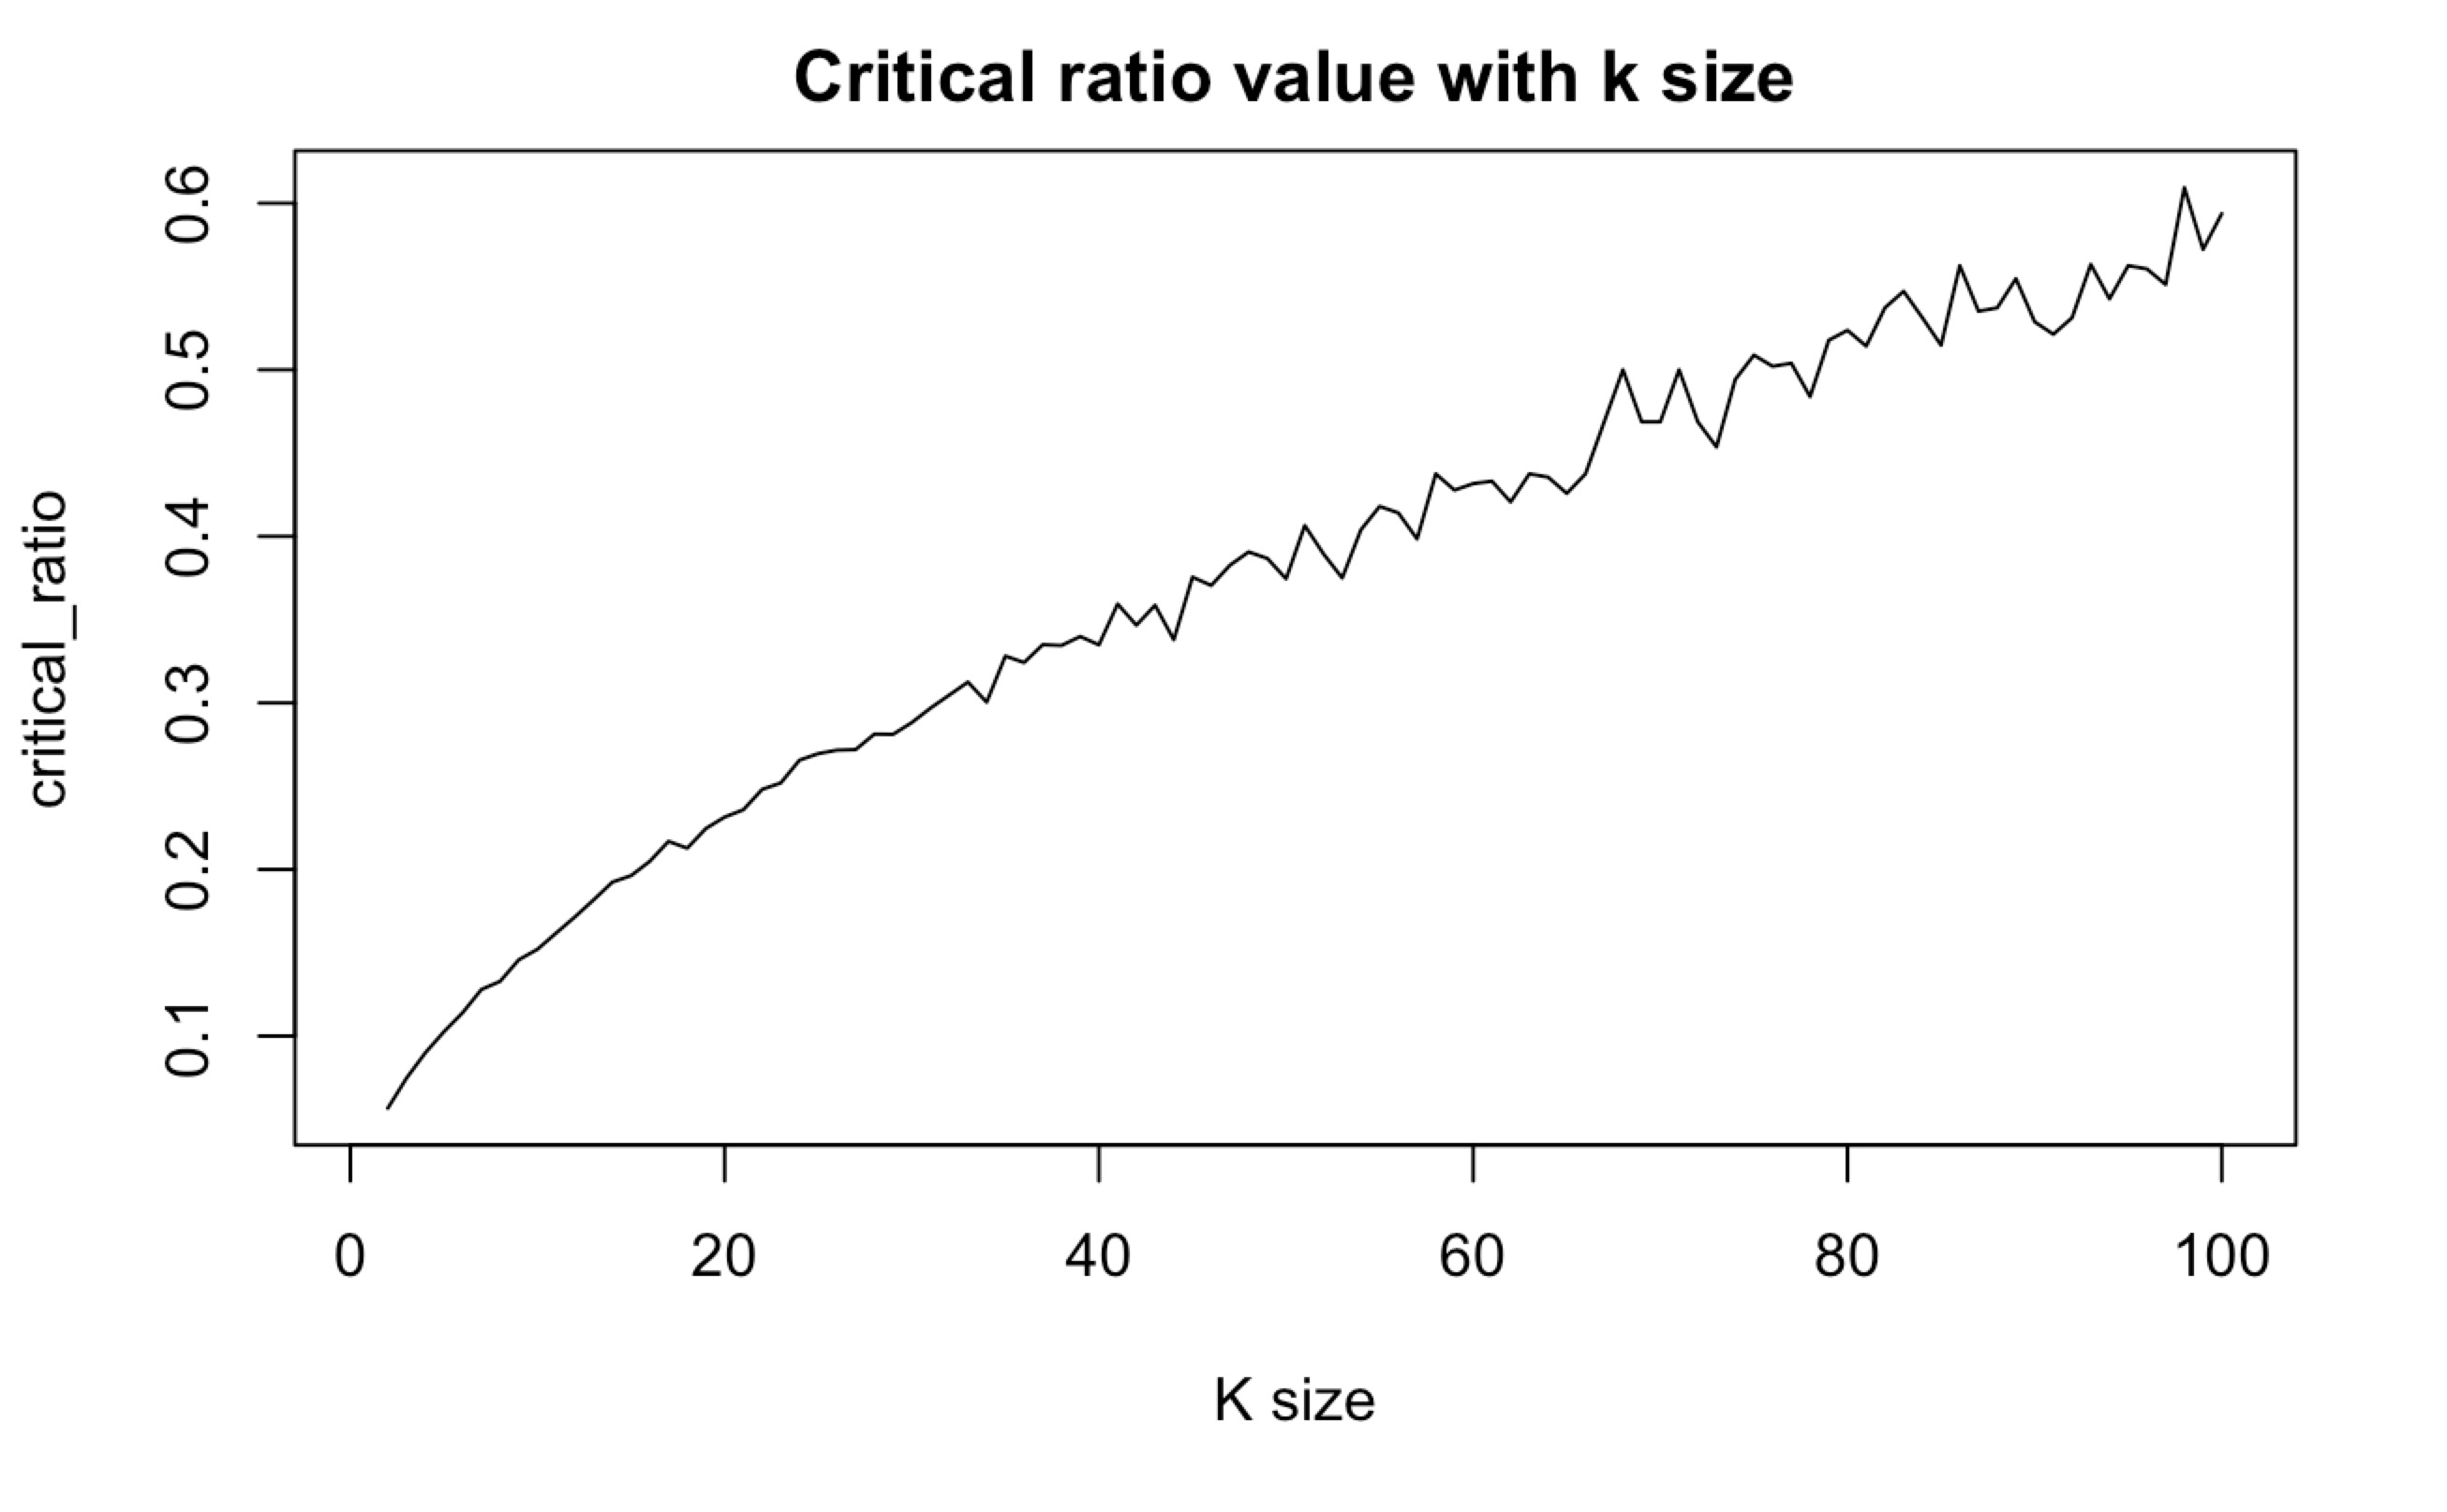
\includegraphics[width=8cm,height=4.5cm]{k}
\caption{Critical Ratio for K}
\end{figure}
\begin{figure}[htbp]
\centering\subfigure[Log K]{
\begin{minipage}{8cm}
\centering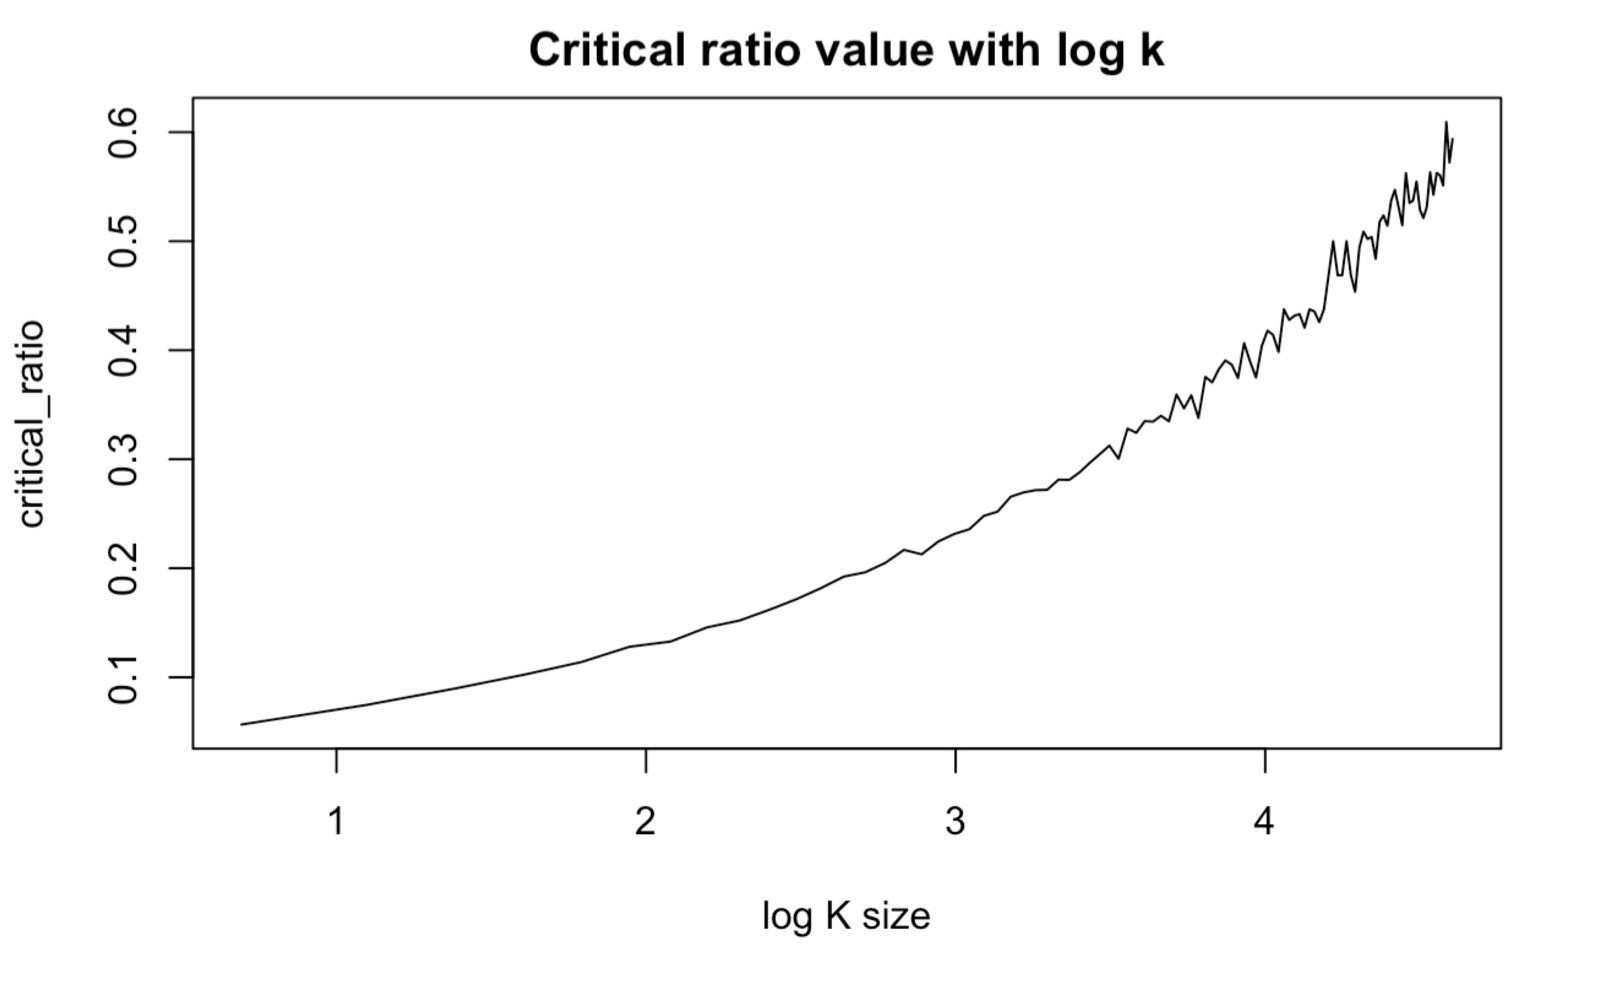
\includegraphics[width=8cm,height=4.5cm]{logk}
\end{minipage}
}
\subfigure[Sqrt K]{
\begin{minipage}{6cm}
\centering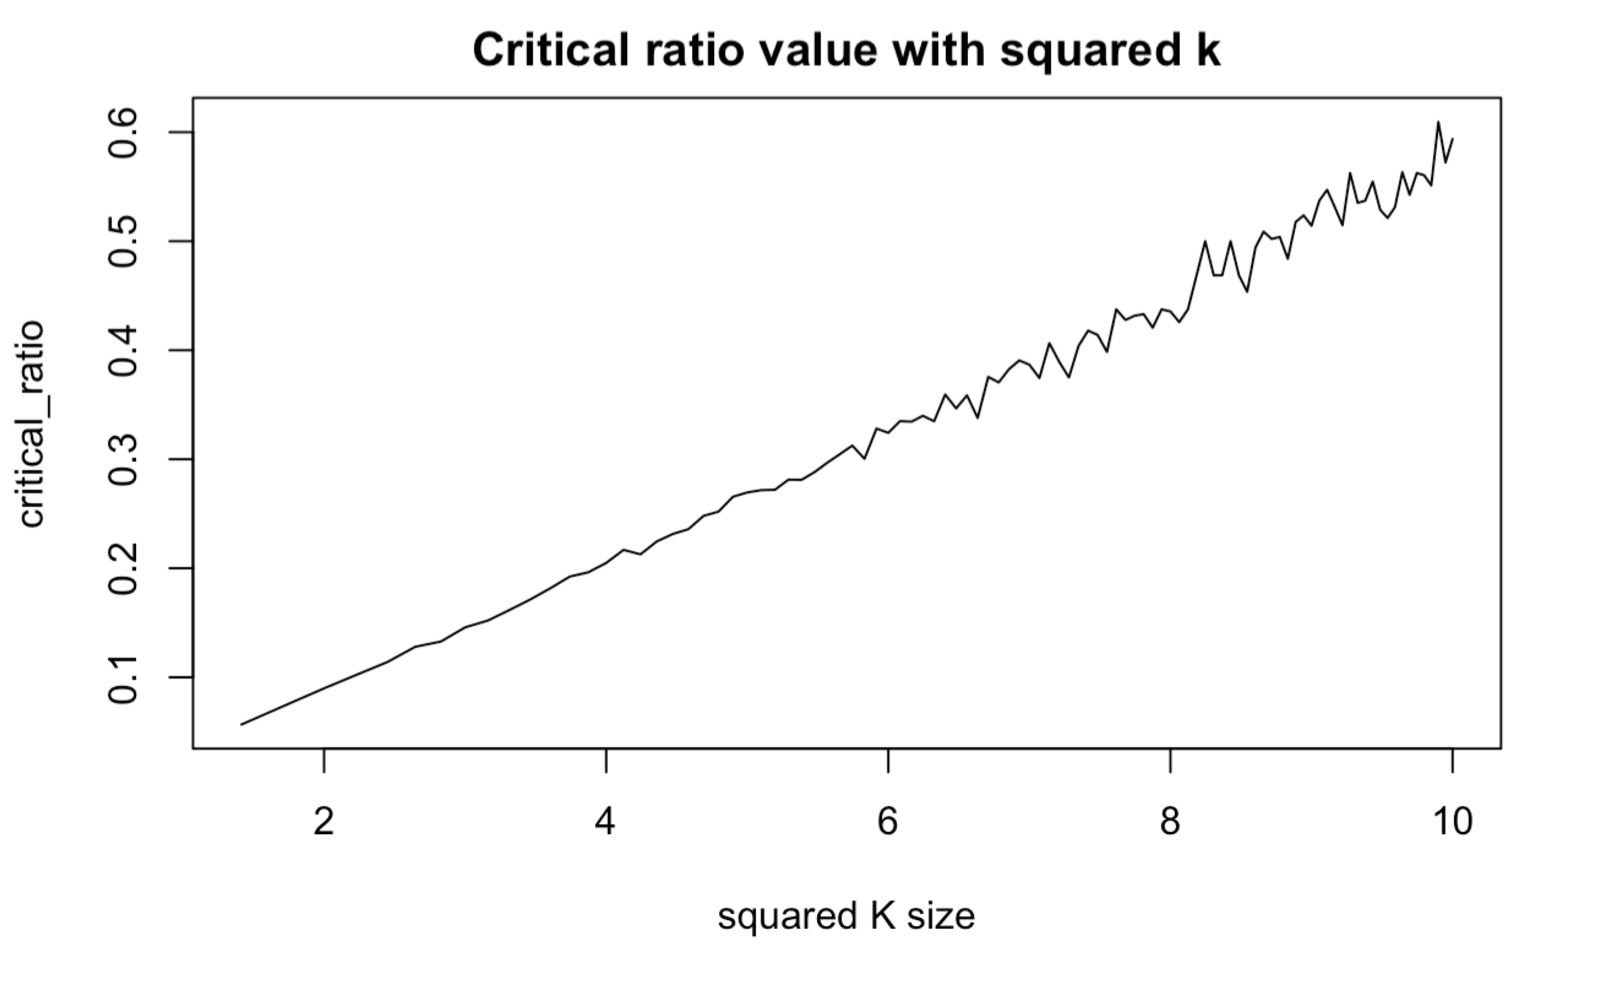
\includegraphics[width=8cm,height=4.5cm]{sqrtk}
\end{minipage}
}
\caption{Logarithm K and squared root K}
\end{figure}
\quad\\
\quad\\
We further apply the linear regression to compare $\sqrt{K}$ and $\log{K}$.\\
\begin{figure}[htbp]
\centering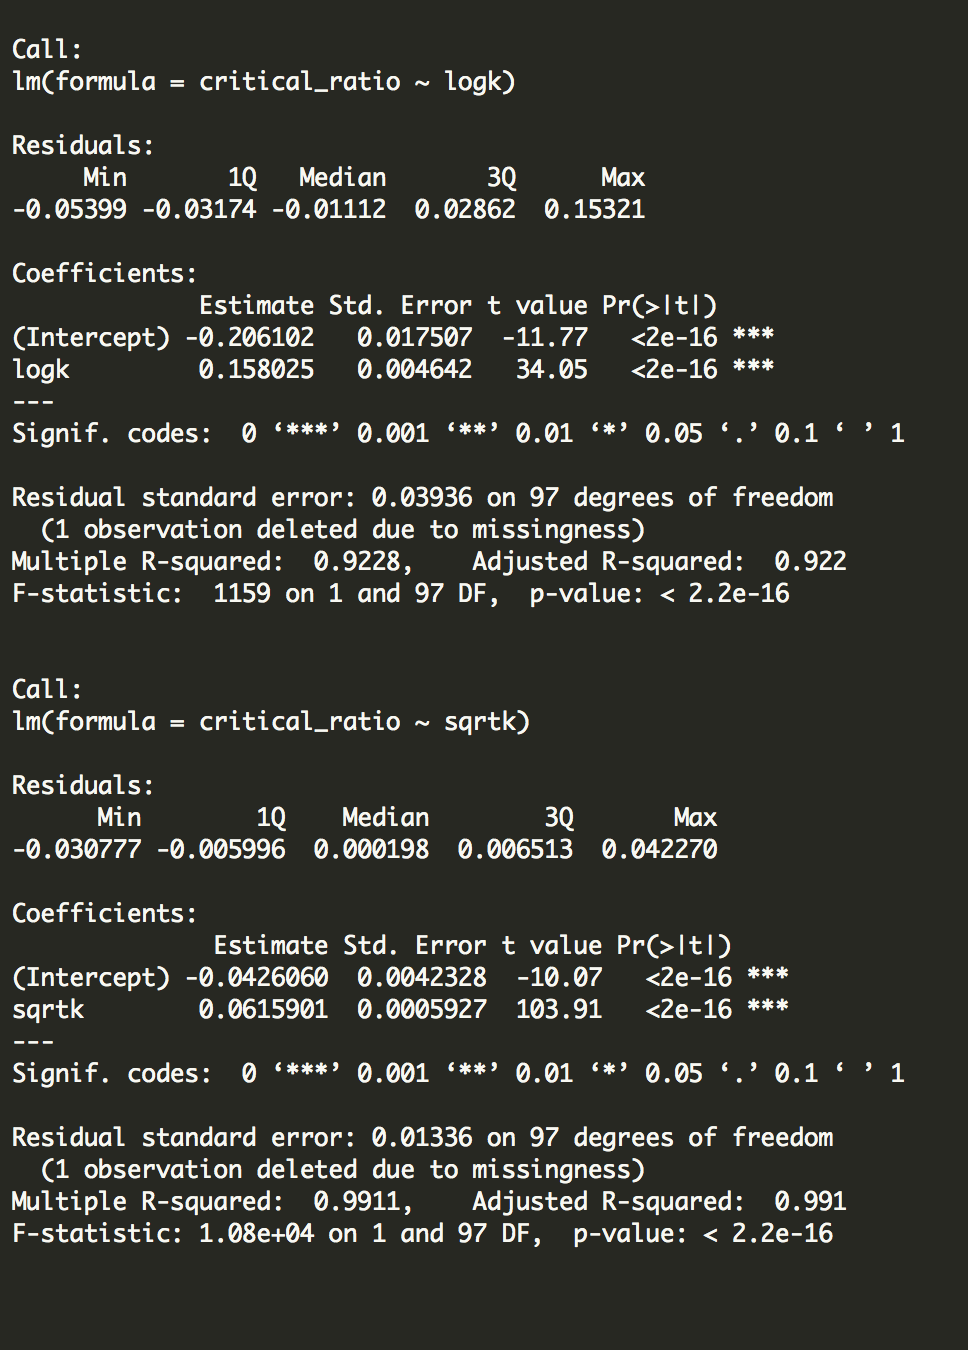
\includegraphics[width=4.3in, height=5in]{reg}
\caption{Regression Summary}
\end{figure}
\quad\\
Note the $\sqrt{K}$ 's $\beta$ coefficient is more statistically significant and larger, while the $r^2$ of log is also larger than $\log{k}$, this supports the reasoning that critical ratio is logarithm increase. In particular, the r squared for  $\sqrt{K}$ model is high as 0.9911, indicating a potential theoretical relationship.



\section{Isotonic Regression}
To make the power non-decreasing, which will be a more reasonable result, we use isotonic regression to the power and get a new plot where the isotonic curve is represented by the red lines. For this plot, we hold $r_k$ and $\sigma$ to be constant while varying $r_1$ and $Y_1$.\\
\begin{figure}[htbp]
\centering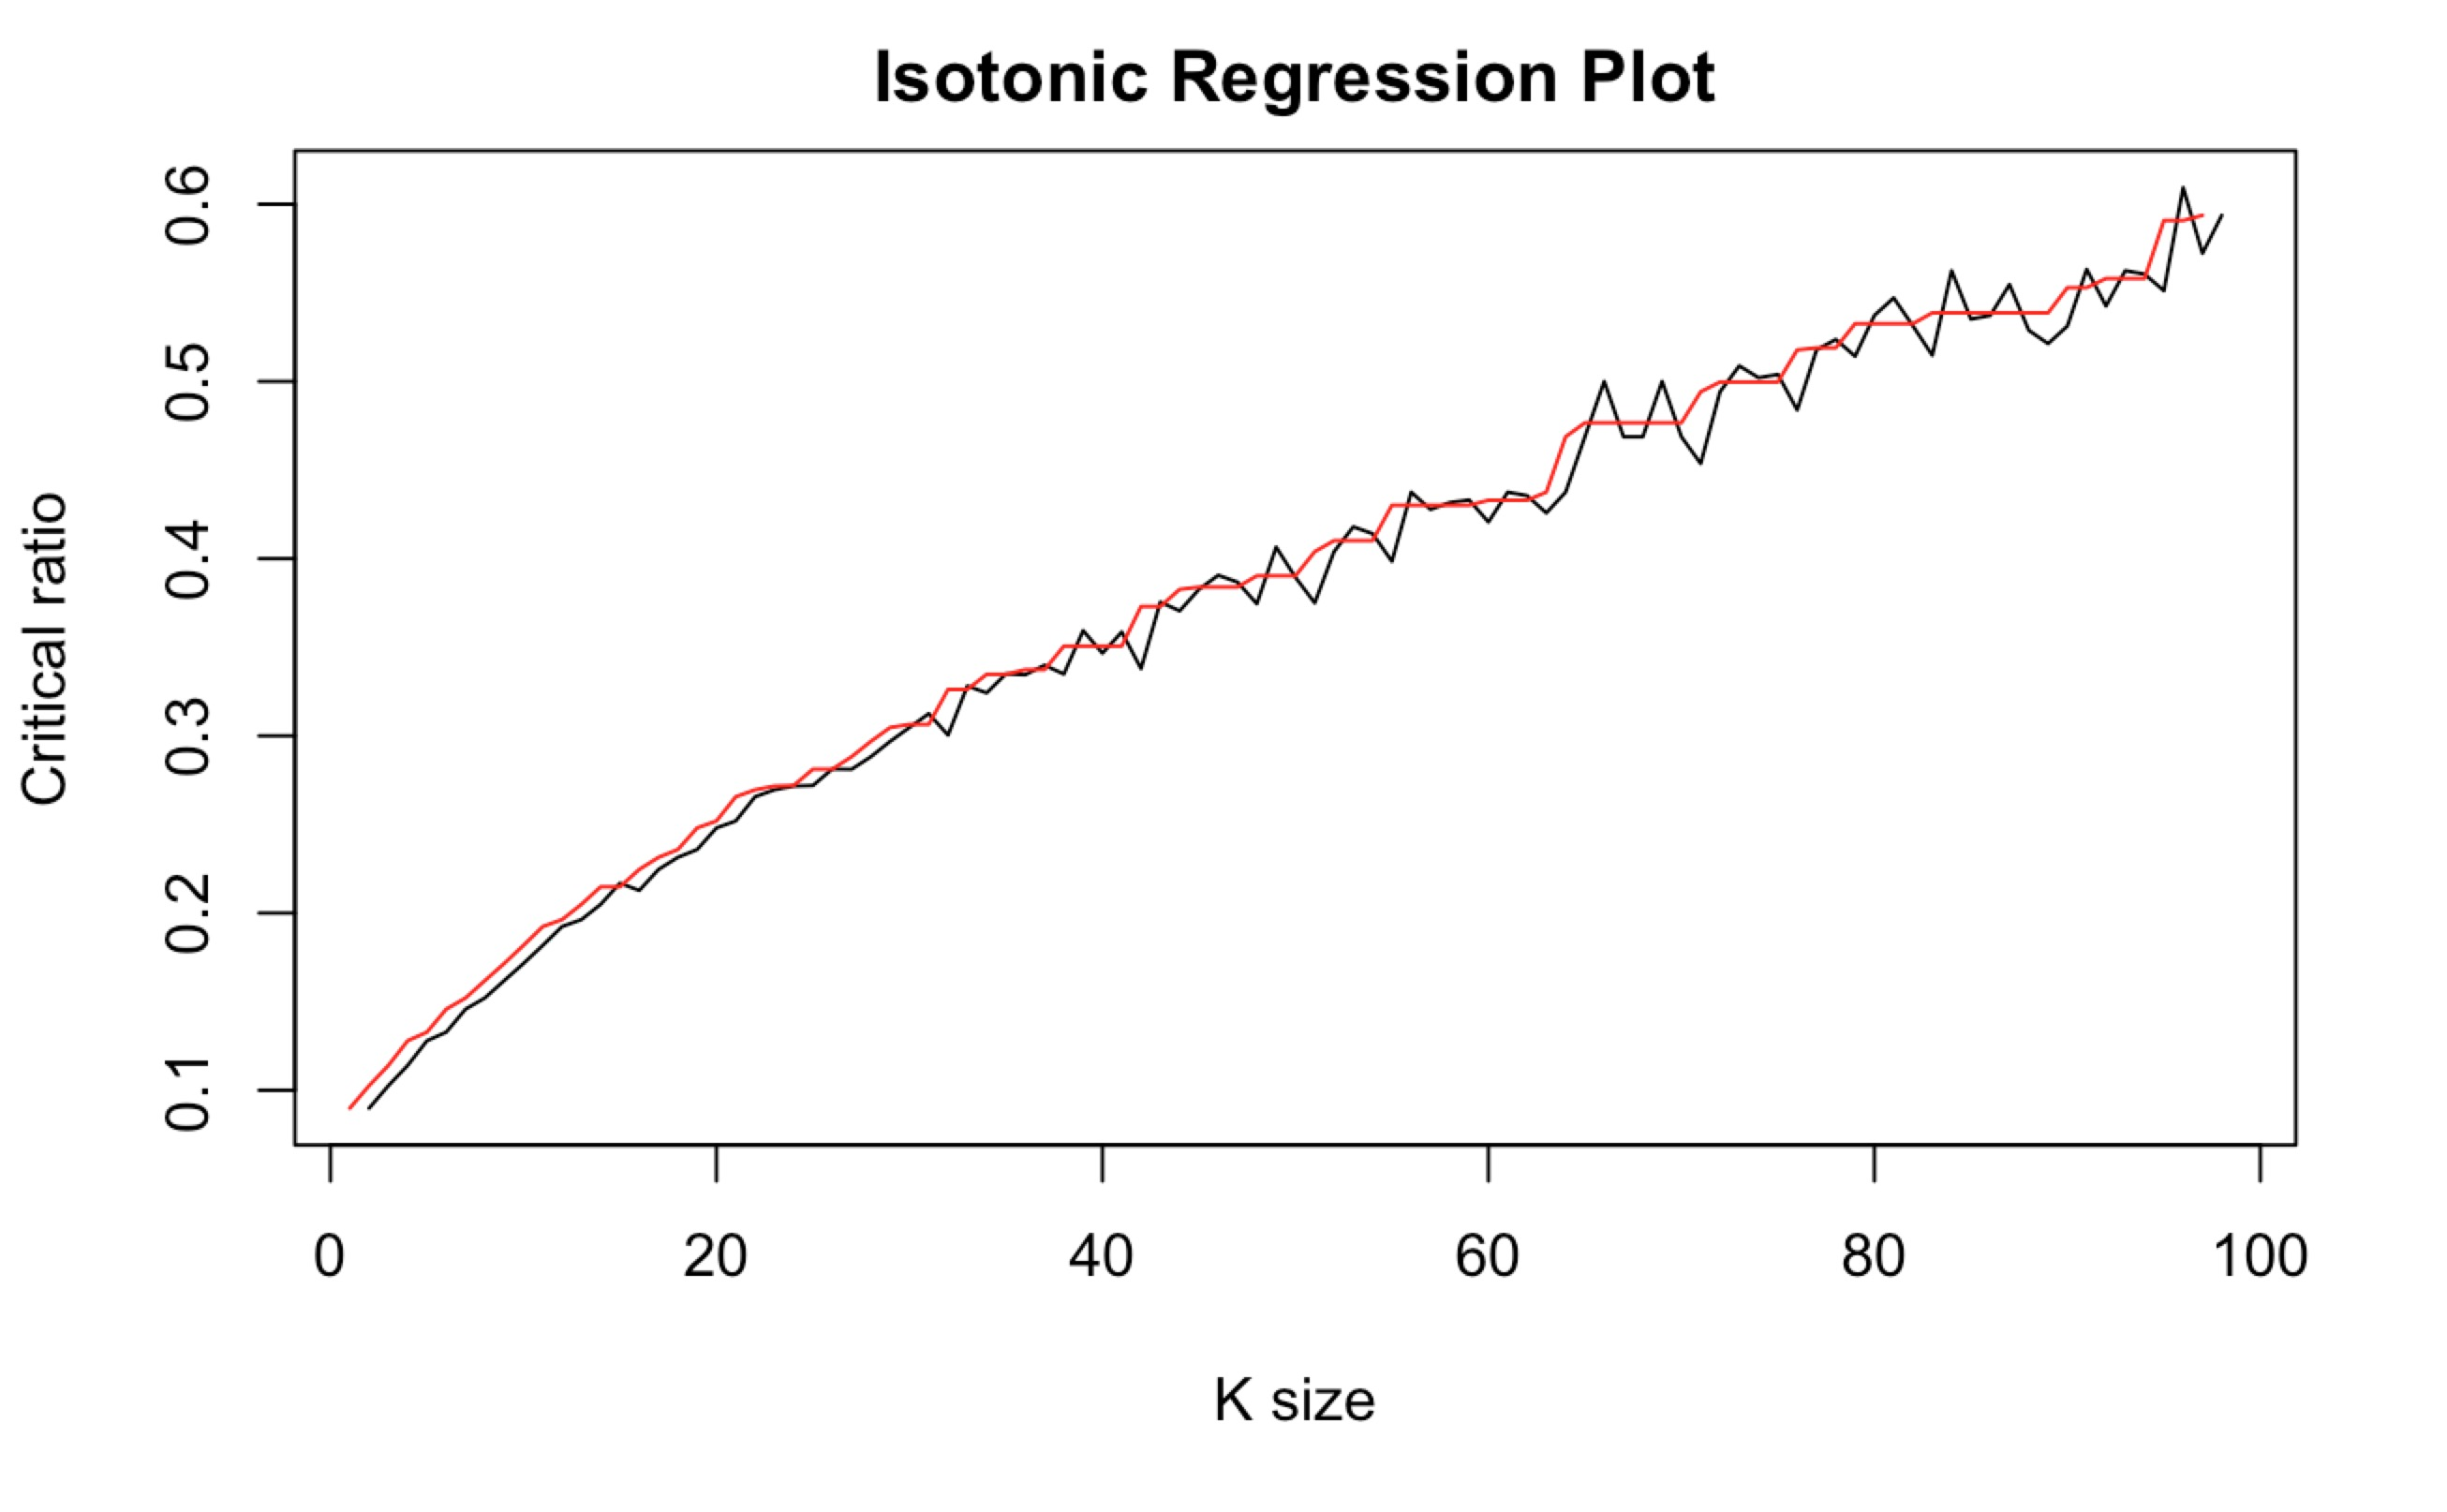
\includegraphics[width=10cm, height=8cm]{iso}
\caption{Isotonic Regression Plot}
\end{figure}
\quad\\
\quad\\
\quad\\
\quad\\
\quad\\
\quad\\
\quad\\
\quad\\
\quad\\
\section{Repetition Times}
To make our analysis much more reasonable, we try to increases the repetition times of our experiment. But the ways to increase the repetition times is very important. Simply just increasing $N$ is actually not the best choice since the $\sigma$ will also increase at the same time, leading to the less reasonable comparison between the experiments. So we come up with other ways to increase the repetition times, in the sense of bootstrap sampling and independent repetition experiments, deriving more sample p-values and taking the mean of them. \\
\quad\\
From a power derivation with one p-value matrix, we could at least get $\frac{N}{K}$ number for getting power. However, given the assumption of independence, we could repeatedly randomly sample to increase the repetition number (rep\_10, rep\_50, rep\_n, boot\_50 increase from 10 times to 50$\times$n times). In addition, we could repeat the whole power derivation process and get more independent results (cv\_10, cv\_50). The results are shown in the following.
\begin{figure}[htbp]
\centering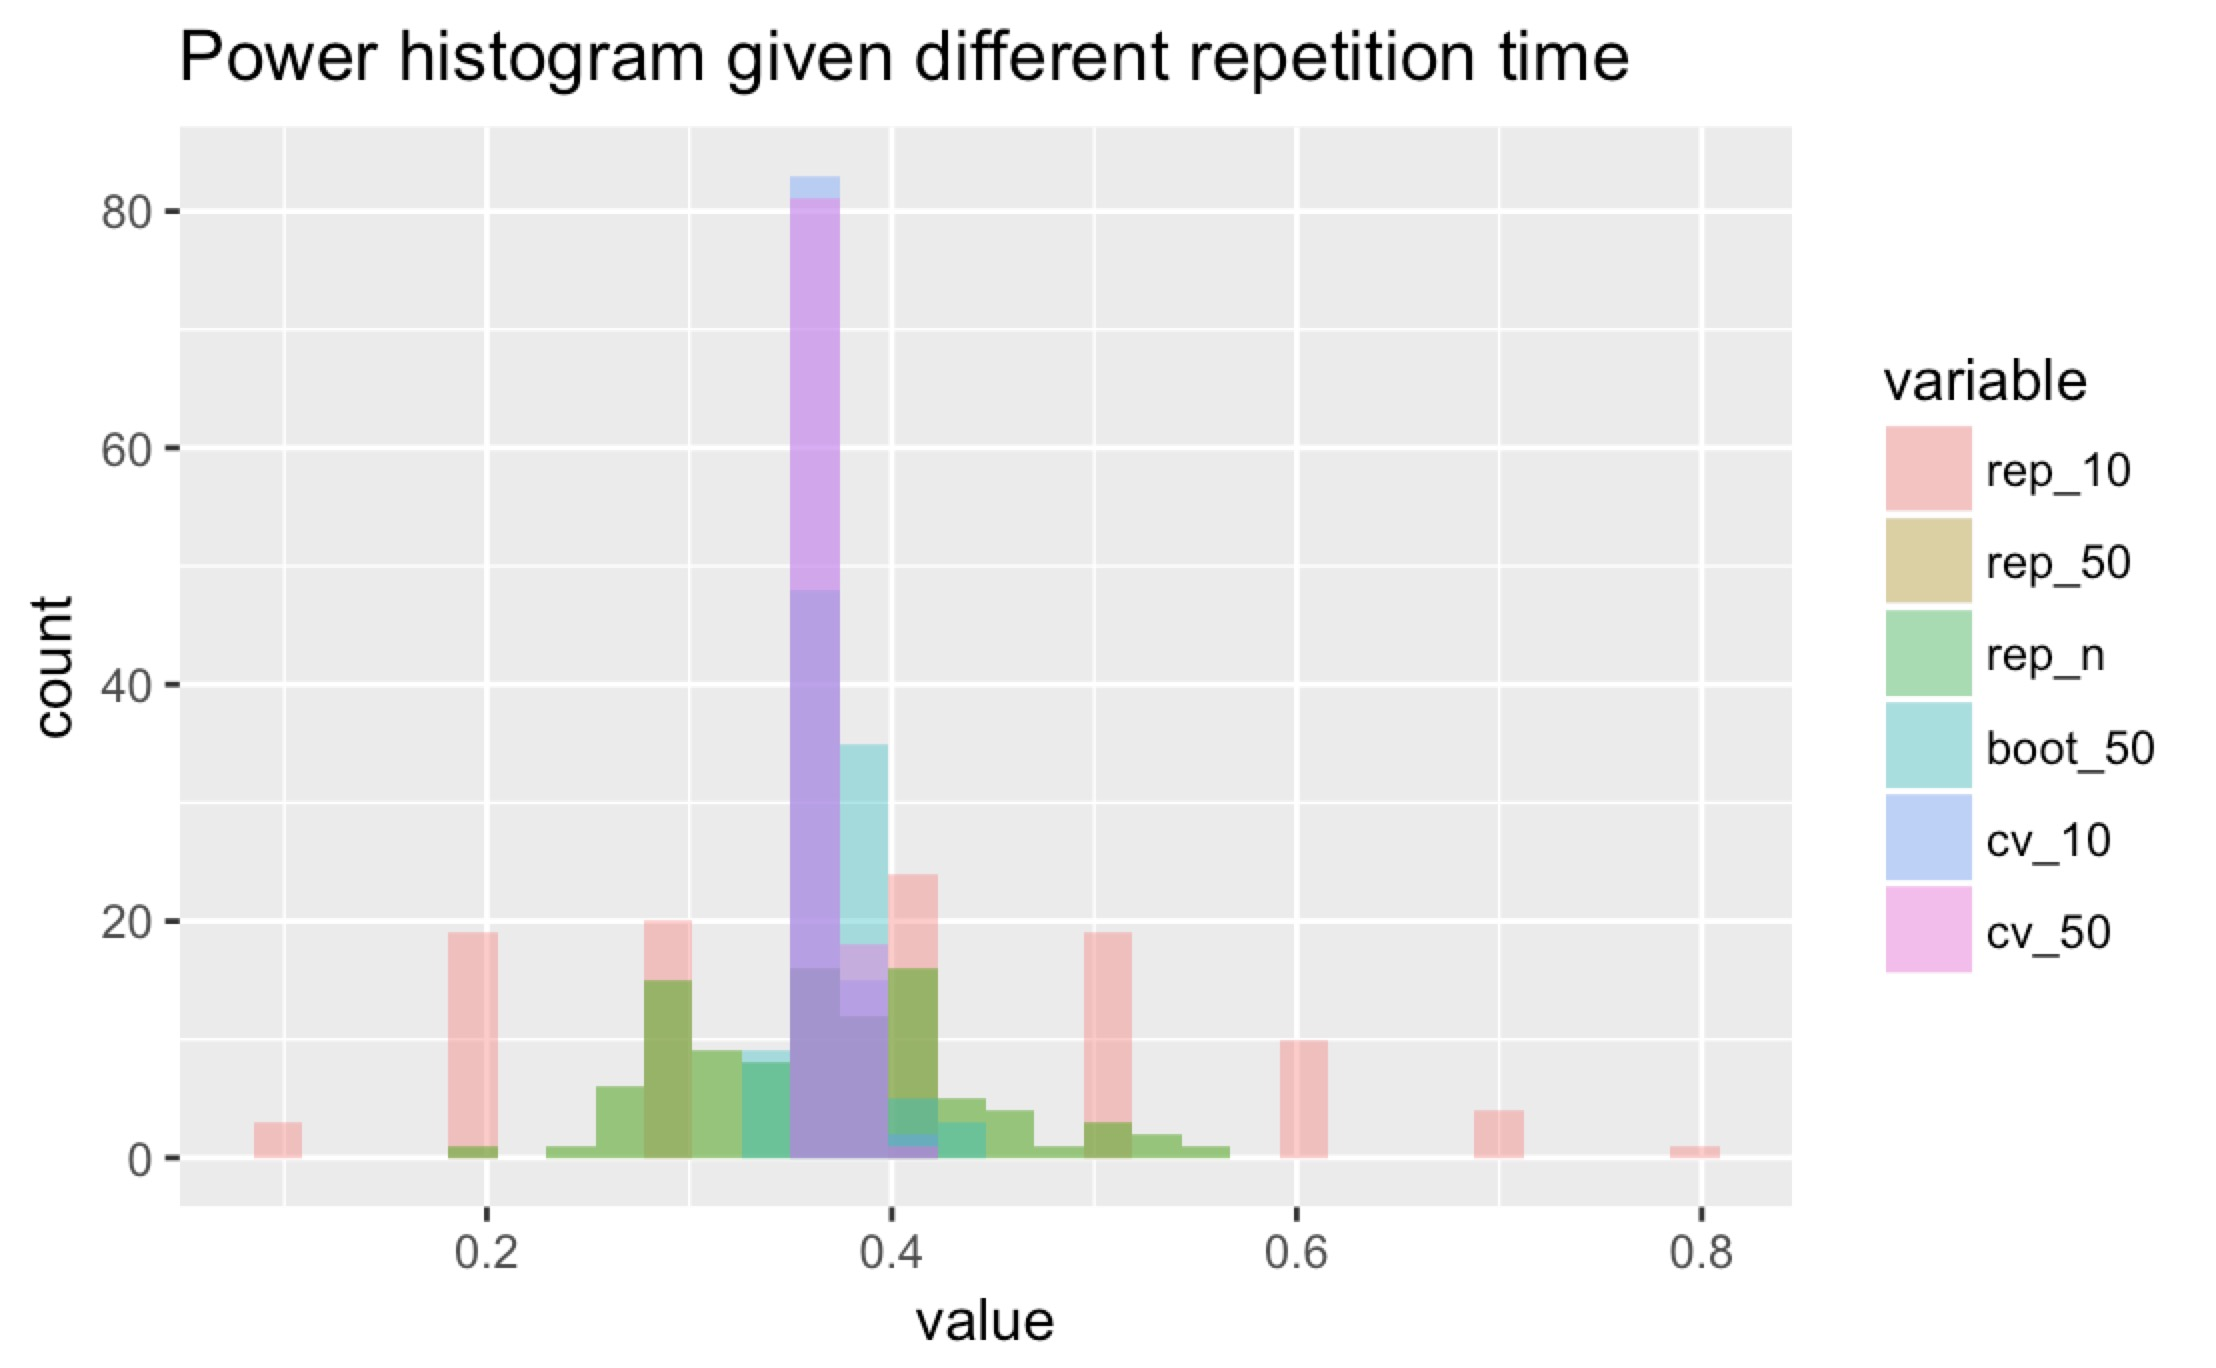
\includegraphics[width=11cm,height=8cm]{hist}
\caption{Power histogram given different ways to increase the repetition times}
\end{figure}
\quad\\
Note as the repetition time increases, the power samples are more closely distributed. And the repeated independent experiment is better off than bootstrap sampling. \\

We next test the power curve given different repetition times.
\begin{figure}[htbp] 
\centering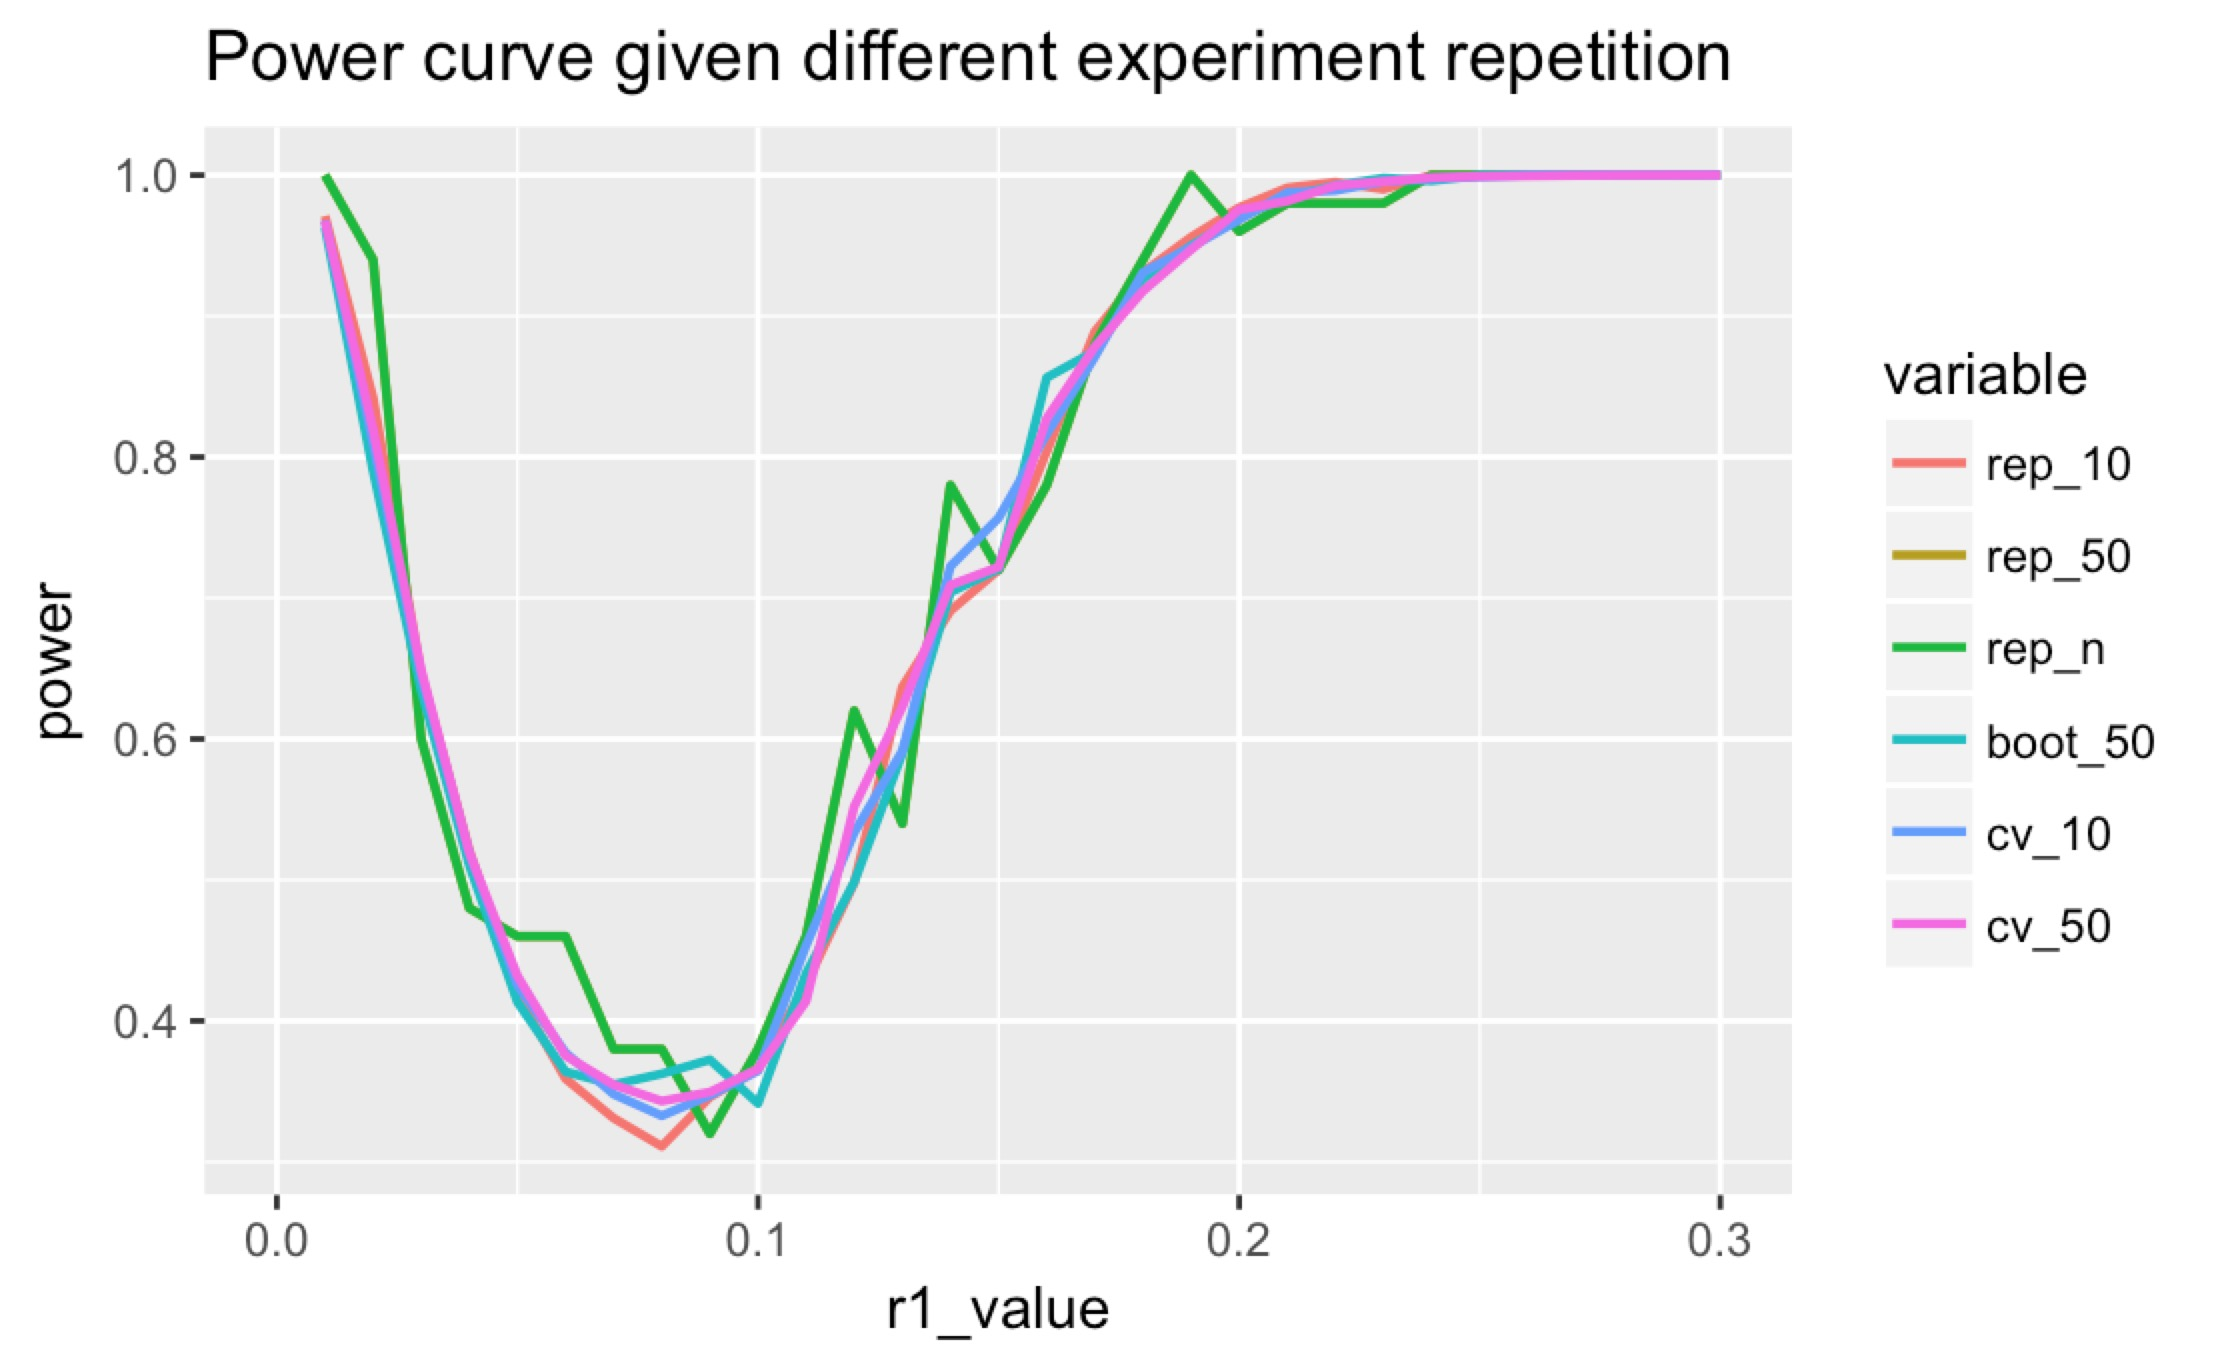
\includegraphics[width=10cm,height=7cm]{line}
\caption{Power curve given different ways to increase the repetition times}
\end{figure}
\quad\\
The independent method (cv\_10 and cv\_50) has more smooth curve than others. Also the variance of bootstrap method is 0.0003649825, while independent repetition is 9.204492e-05  and 4.950972e-05 respectively for 10 times and 50 times. Since the 50 times are much time costing than 10 times while the disparity of the two is not that much, we choose the repetition time of 10 as our applied power derivation choice.


\section{Scaling}
For this part, we hold $r_1=\frac{Y_1}{\sigma_1}$ and $r_k=\frac{\sigma_k}{\sigma_1}$ to be constant, which means that $\frac{Y_1}{\sqrt{\sigma_1^2+\sigma_k^2}}$ is constant. Under this condition, we try to plot Y ranging from 0 to 1 by 0.01 step, as well as 1.2Y, 1.5Y and 2Y. But at the same time, we find the the ratio $r_1$ also has significant impact on the power, leading to the different power pattern of the plot. So we also make different plots by $r_1$ ranges from 0.01 to 0.3.\\
\begin{figure}[htbp]
\centering\subfigure[]{
\begin{minipage}{8cm}
\centering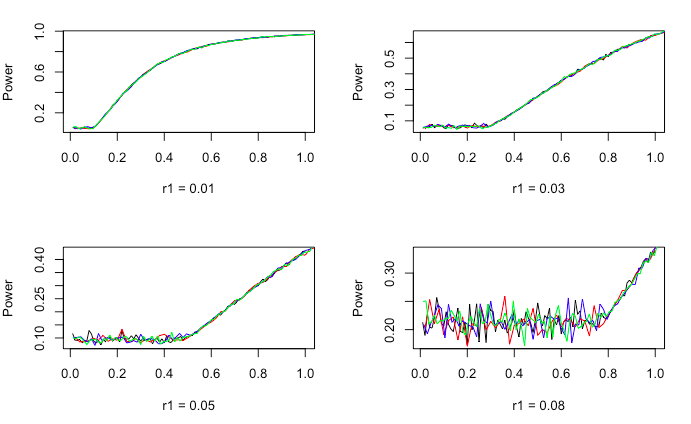
\includegraphics[width=8cm,height=6.2cm]{sca1}
\end{minipage}
}
\subfigure[]{
\begin{minipage}{6cm}
\centering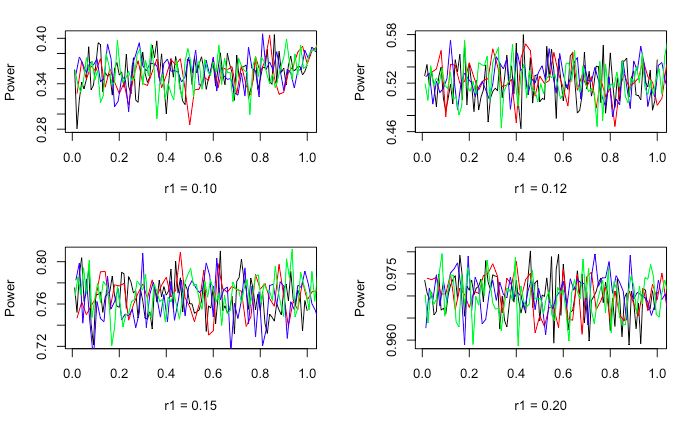
\includegraphics[width=8cm,height=6.2cm]{sca2}
\end{minipage}
}
\caption{Scaling Plot}
\end{figure}
\begin{figure}[htbp]
\centering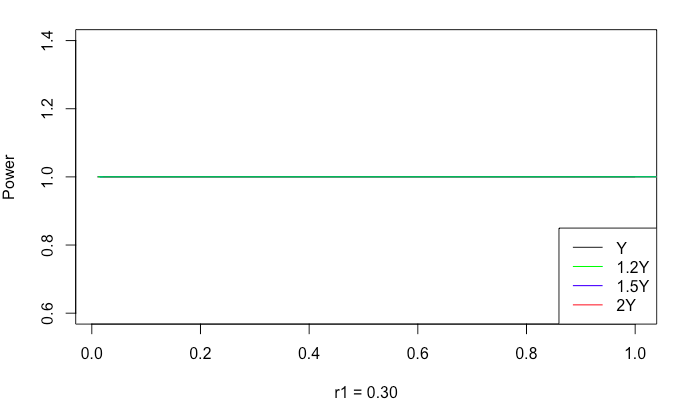
\includegraphics[width=10cm,height=7cm]{sca3}
\caption{\label{1}Scaling Plot}
\end{figure}
\quad\\
The good news is that when we hold $r_1$ and $r_k$ constant, no matter how $Y_1$ changes, the power pattern seems to be the same. But from the plot we can see that when $r_1=0.01$, it turns out to be a "S-shape" curve; in $r_1=0.03$ and $r_1=0.05$, the horizontal part of the curve tends to oscillates more and the power, from the y-axis we can see, becomes smaller. When $r_1=0.08$, the plot seems all to be the horizontal oscillating part, and the power is around the smallest value, where maximum equals to around 0.3. When $r_1$ ranges from 0.1 to 0.2, we can see that the power all oscillates and increases closed to 1. And from Figure \ref{1}, we can see that all power equals to 1.\\
\quad\\
To the further discussion of $r_1$, we hold $Y_1$ constant while varying $r_1$ to see its power pattern as follow.\\
\begin{figure}[htbp]
\centering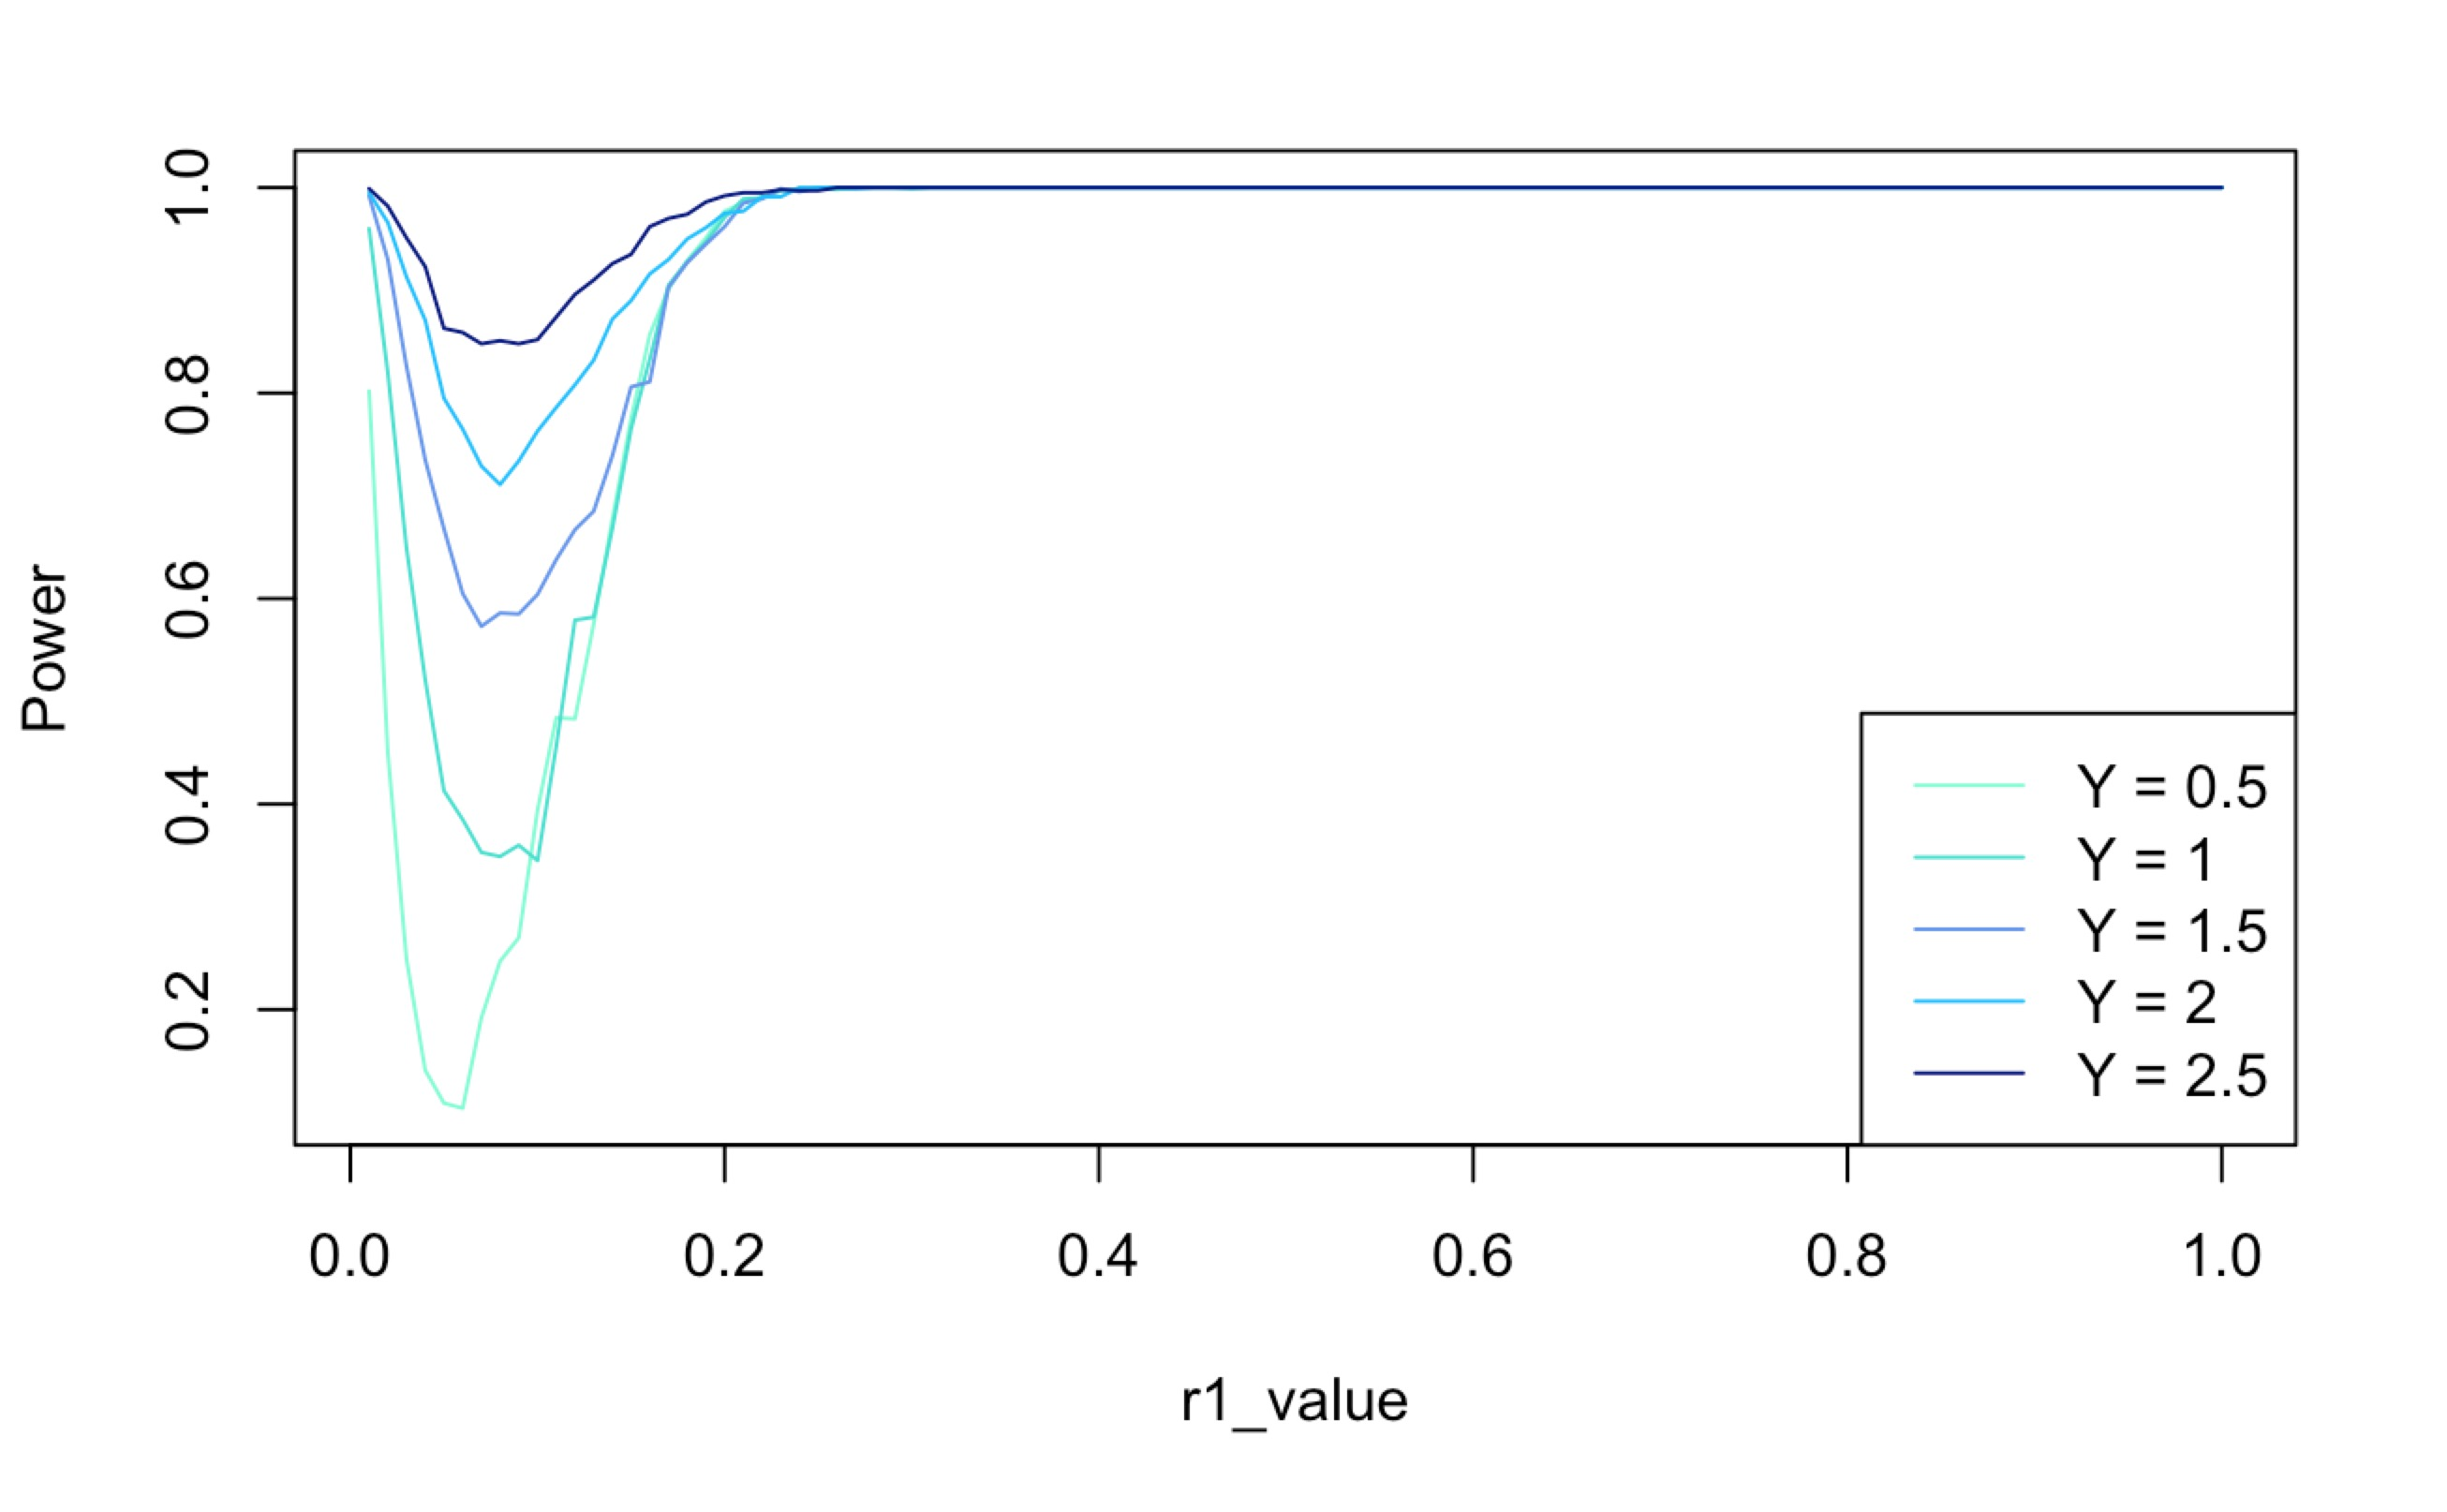
\includegraphics[width=11cm,height=8cm]{r1}
\caption{$r_1$ Plot}
\end{figure}
\quad\\
We can see that it corresponds to the plot before as the power first decreases and then increases. And if $Y_1$ increases, the power will become more stable.\\


\section{P-combined Analysis}
Before, we take the minimum of p-values to generate p\_combined value, and this time, we take different ways to generate p\_combined by taking the maximum, median and mean values. Also, we take treatment size $K$ into consideration.
\begin{figure}[htbp]
\centering\subfigure[K=2]{
\begin{minipage}{8cm}
\centering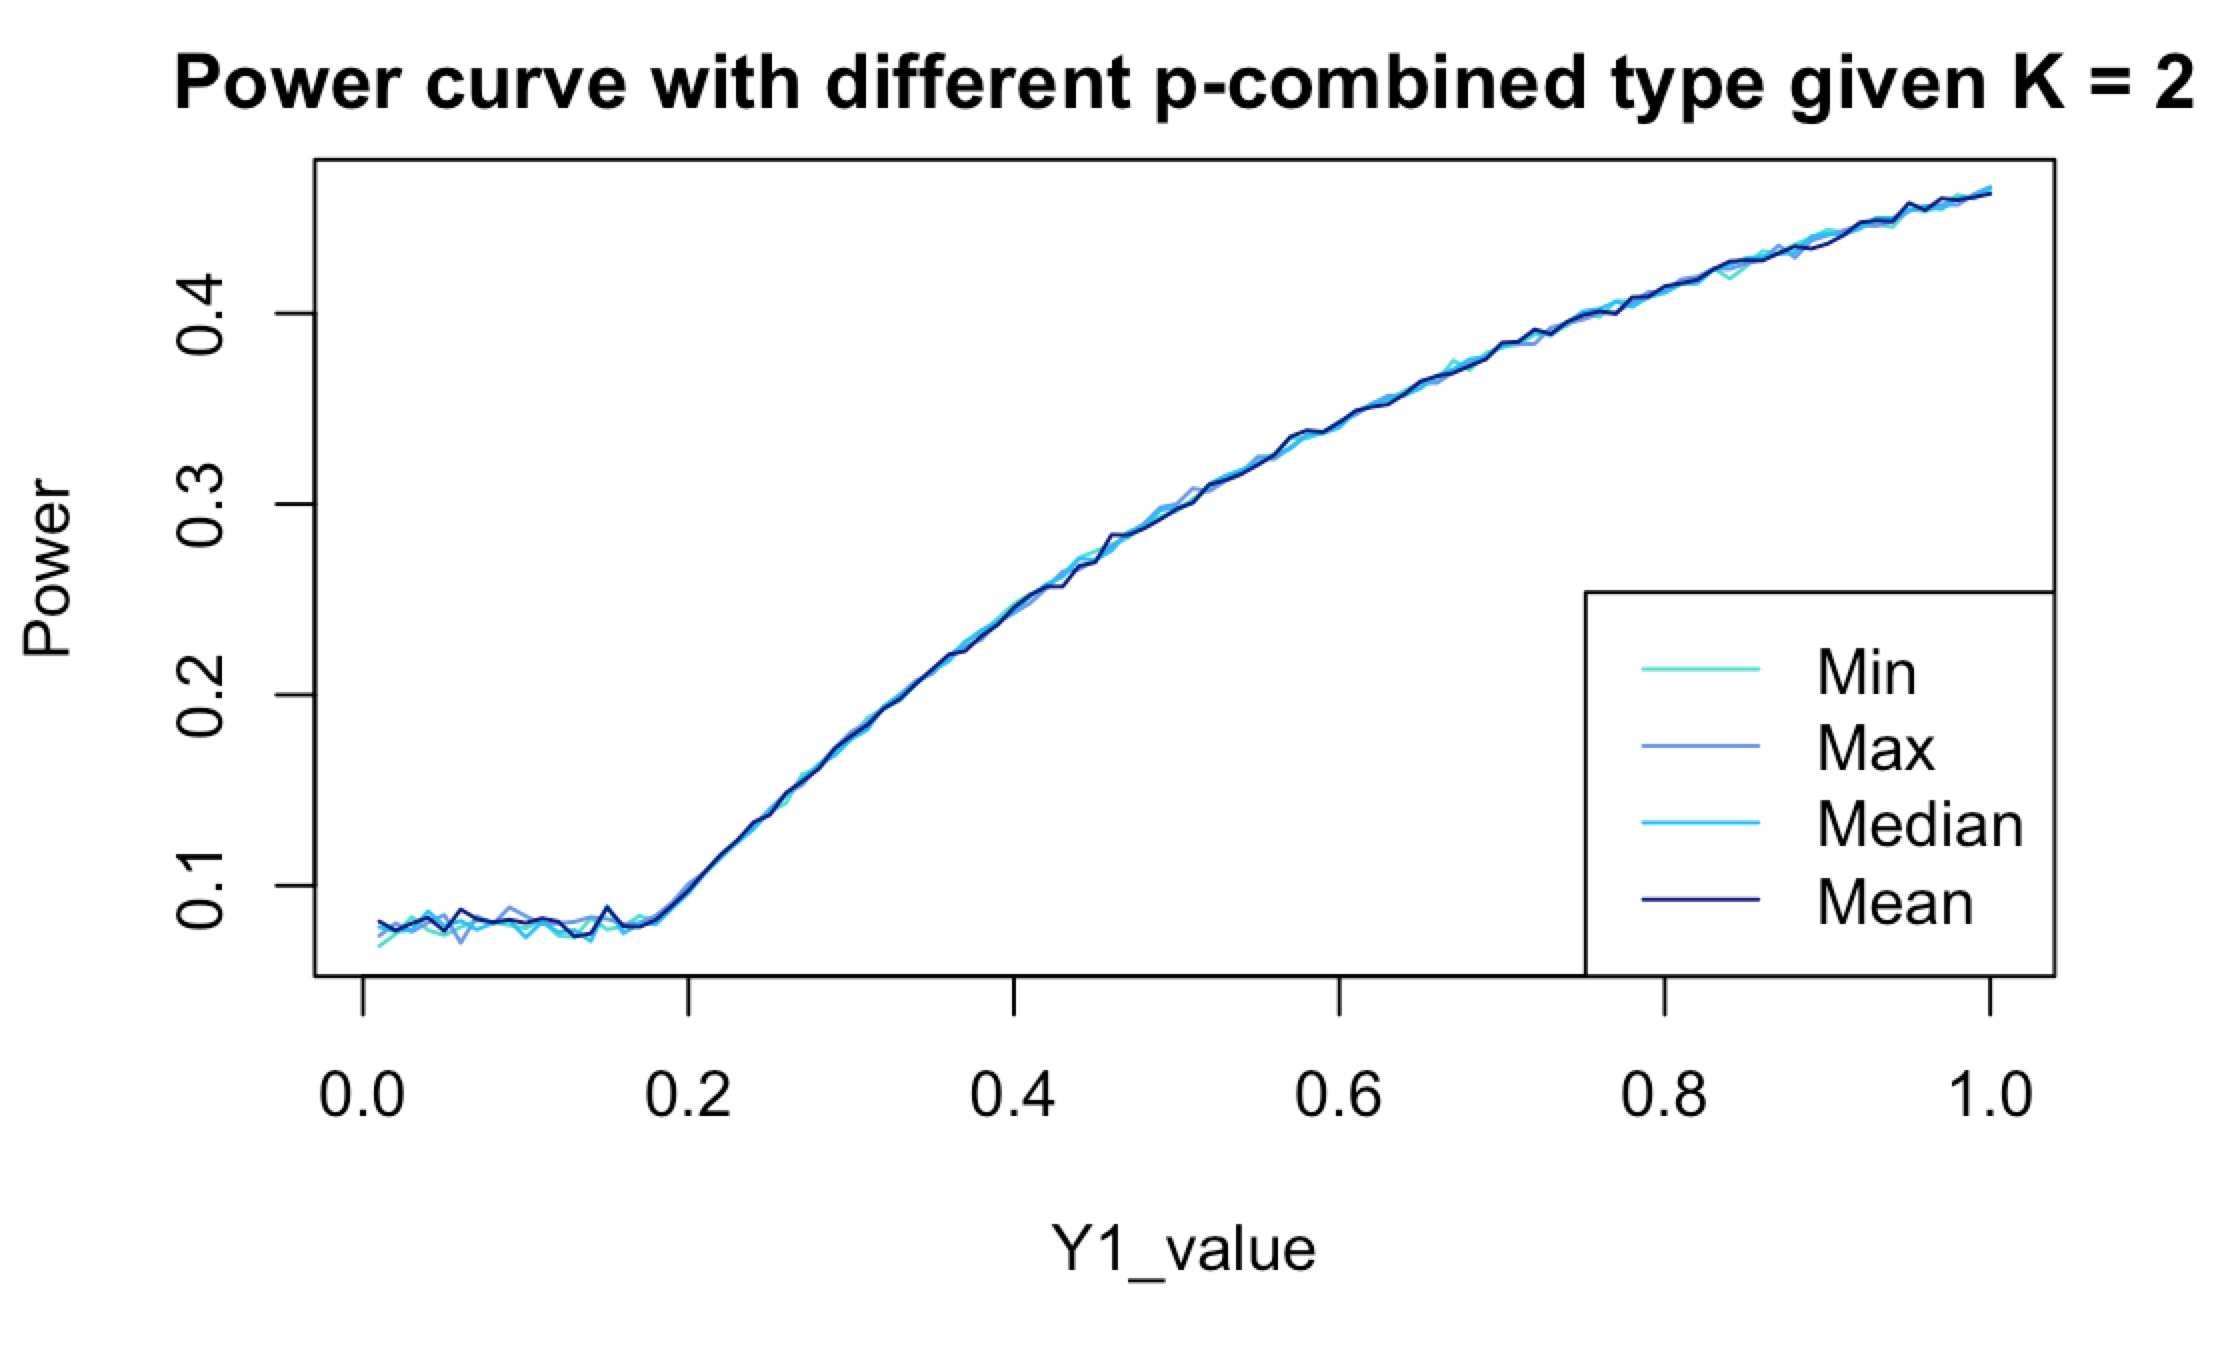
\includegraphics[width=8cm,height=6.5cm]{2}
\end{minipage}
}
\subfigure[K=3]{
\begin{minipage}{6cm}
\centering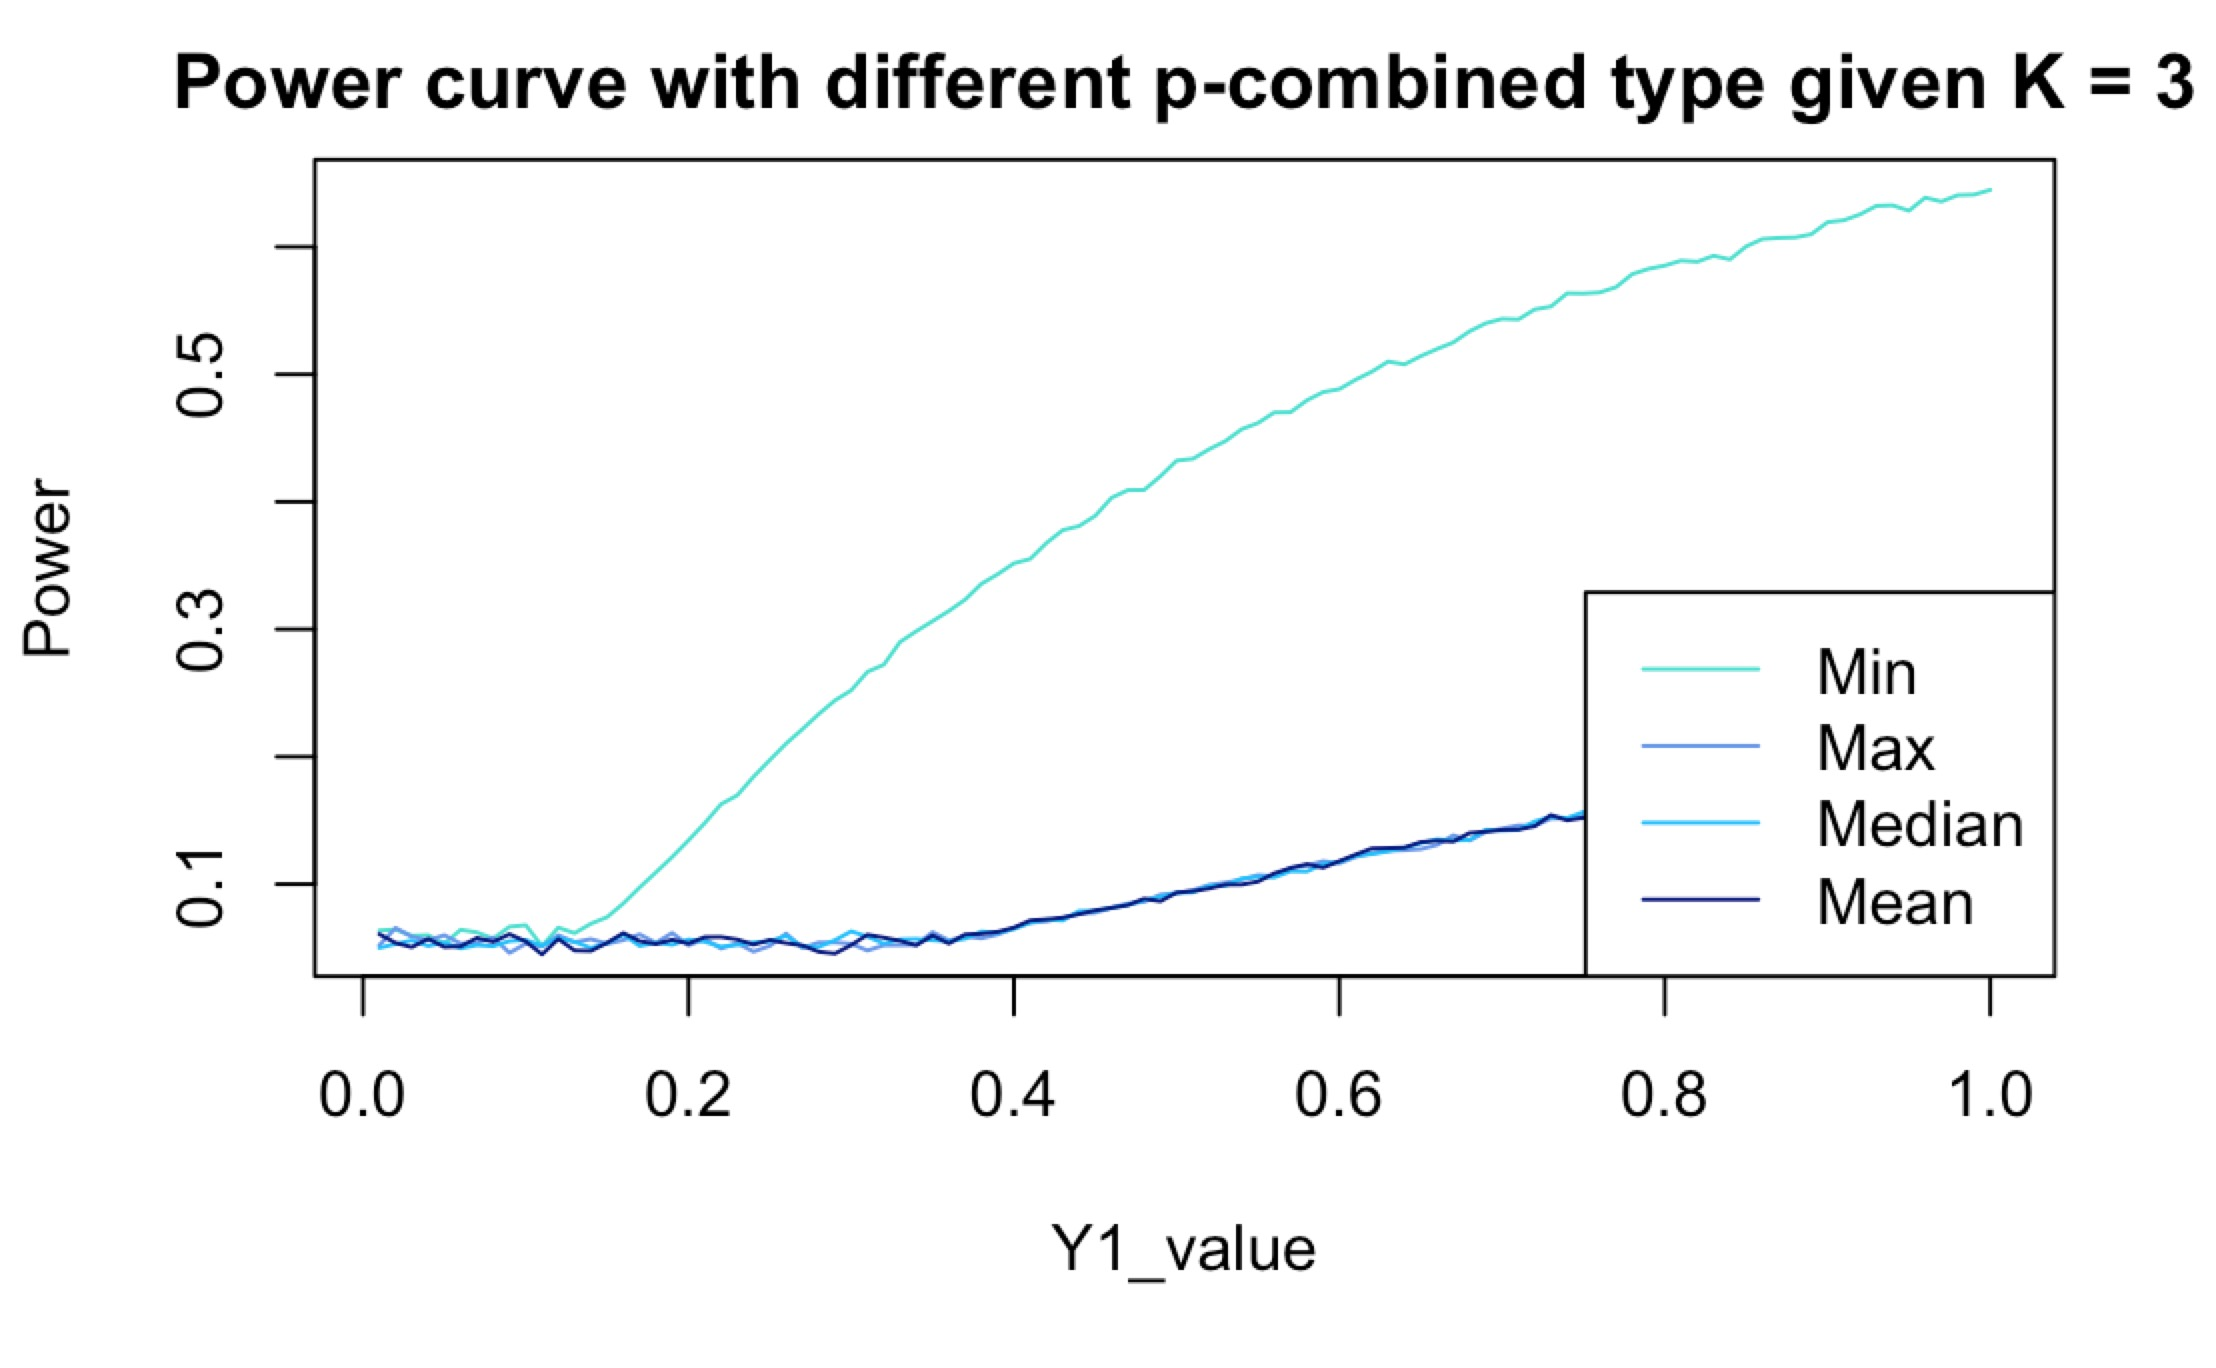
\includegraphics[width=8cm,height=6.5cm]{3}
\end{minipage}
}
\caption{Power plot of different type of p\_combined}
\end{figure}
\begin{figure}[htbp]
\centering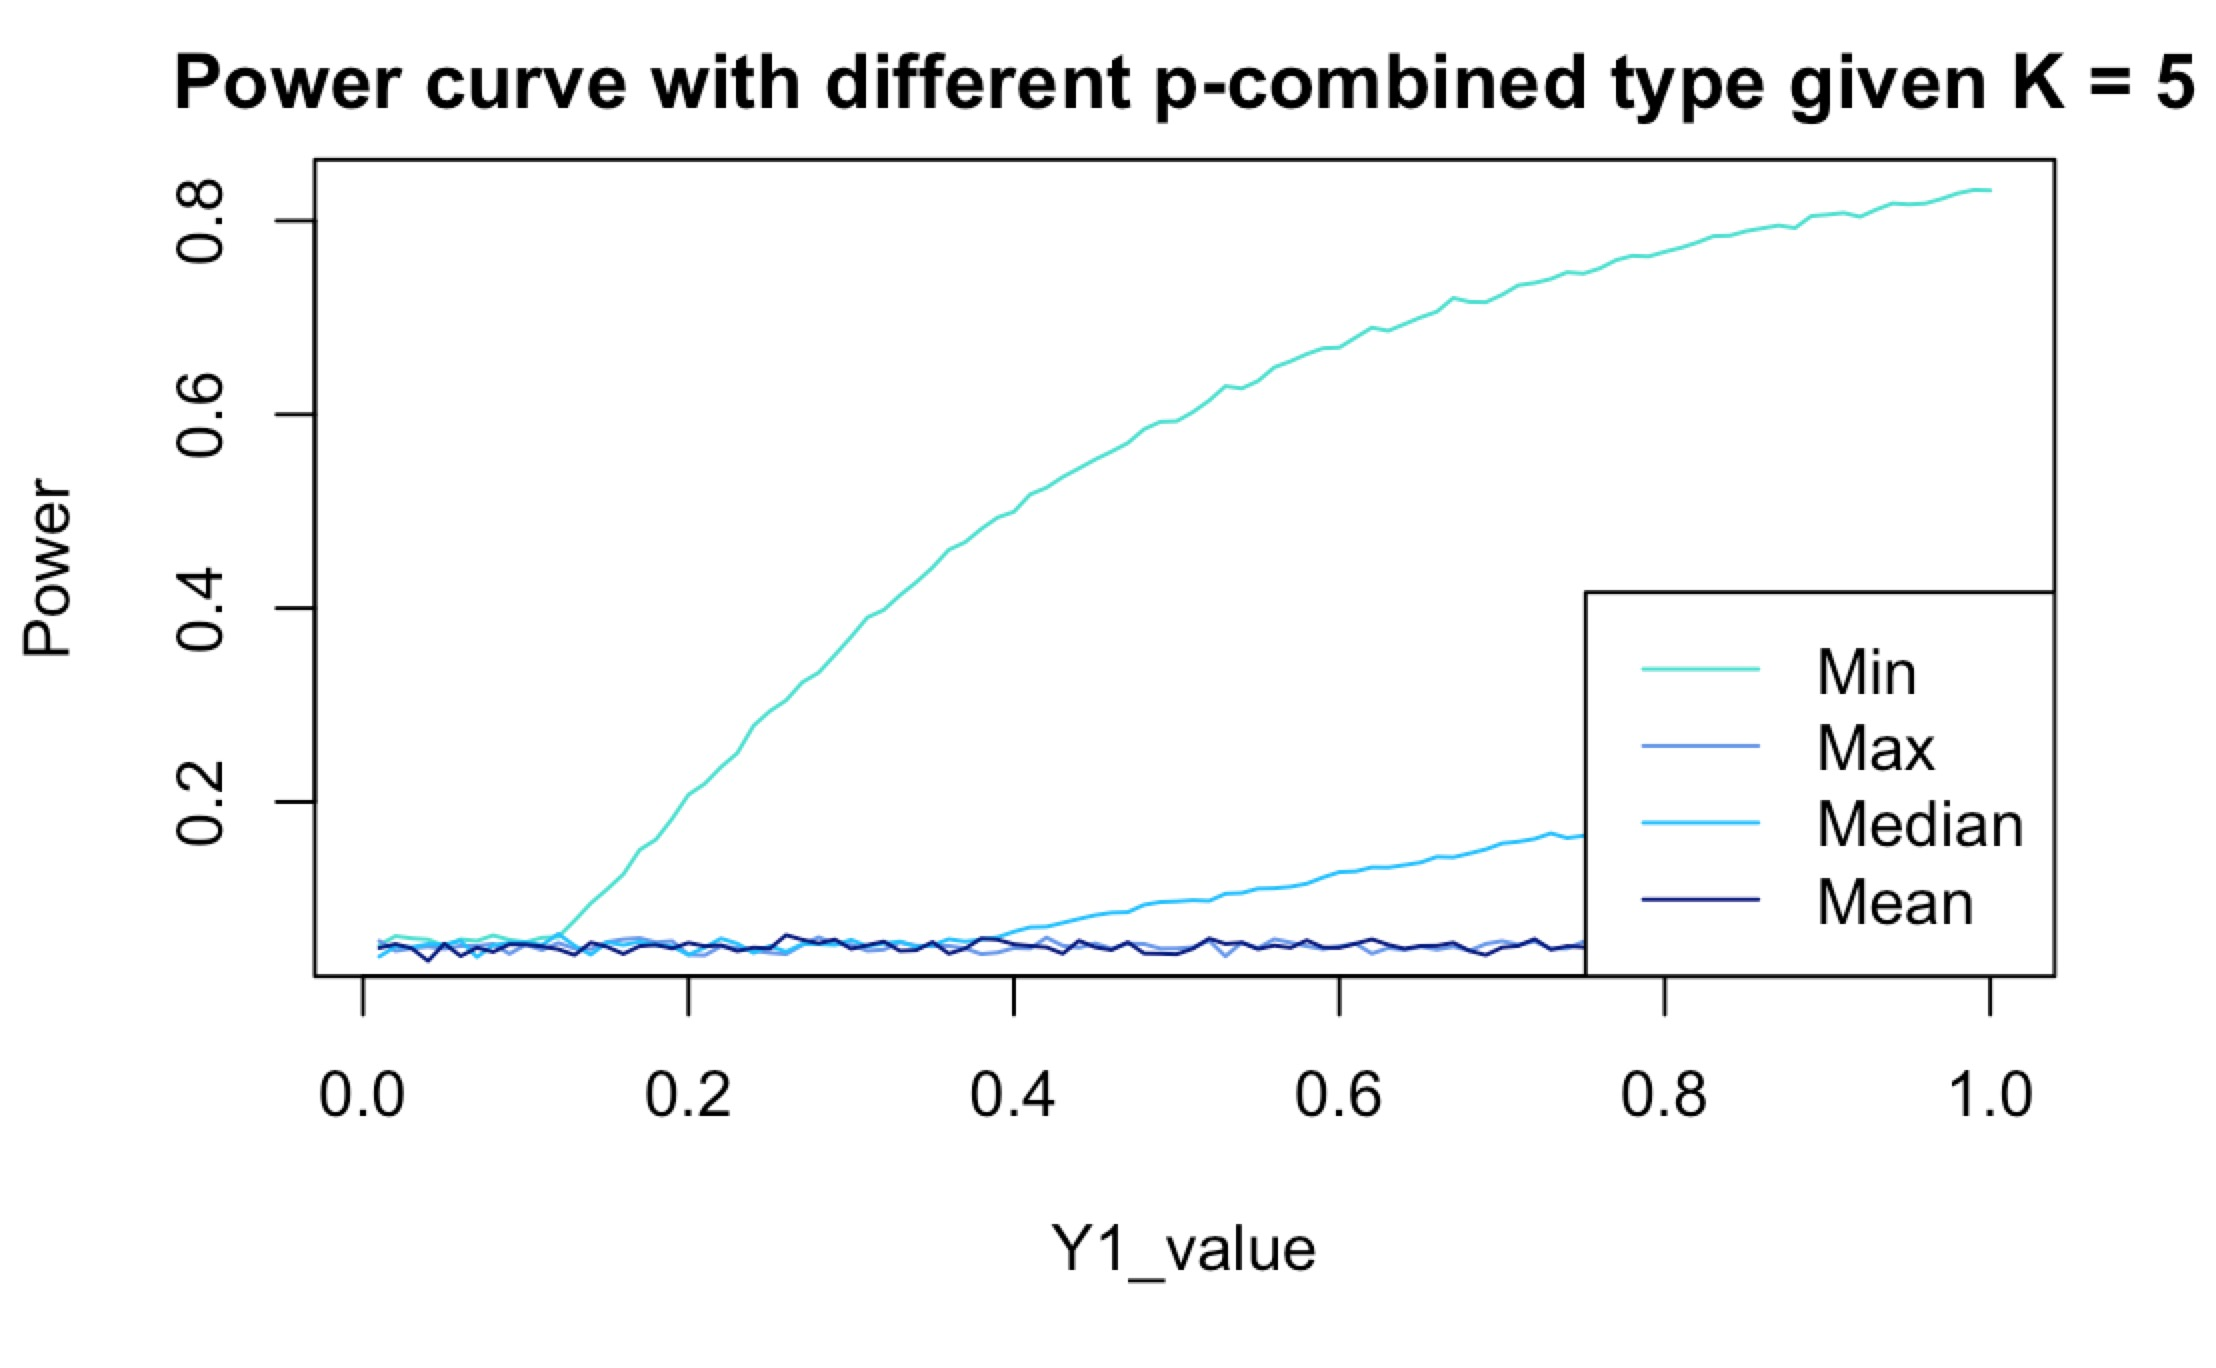
\includegraphics[width=10cm,height=7cm]{5}
\caption{Power plot when K=5 by different type of p\_combined}
\end{figure}
\quad\\
From the plot we can see that as $K=2$, all four types of p\_combined seems to have the same pattern. But when $K$ increases to 3, the minimum still keeps the "S-shape" curve but other three curves become lower. When $K=5$, actually including all values bigger than 5 according to our experiments, the minimum curve still keeps its pattern; the maximum and mean curve just not increase any more and stay horizontally; the median curve has a small increasing trend, a little higher than the mean and maximum curve but much lower than the minimum curve. So we can see the the minimum curve is the most stable one.


\end{document}










